\documentclass{article}


\usepackage{arxiv}

\usepackage[utf8]{inputenc} % allow utf-8 input
\usepackage[T1]{fontenc}    % use 8-bit T1 fonts
\usepackage{hyperref}       % hyperlinks
\usepackage{url}            % simple URL typesetting
\usepackage{booktabs}       % professional-quality tables
\usepackage{amsfonts}       % blackboard math symbols
\usepackage{xfrac}       % compact symbols for 1/2, etc.
\usepackage{microtype}      % microtypography
\usepackage{array}
\usepackage{graphicx}
\graphicspath{ {./images/} }
\usepackage{algorithm}
\usepackage{algorithmic}

\title{A Review of Lossless Data Compression Algorithms}


\author{
	Aditya Meharia\\
	School of Computer Engineering\\
	Kalinga Institute of Industrial Technology\\
	Bhubaneswar, India 751024 \\
	\texttt{adityameharia14@gmail.com} \\
  	%% examples of more authors
	\And
   	Junaid H. Rahim\\
	School of Computer Engineering\\
	Kalinga Institute of Industrial Technology\\
	Bhubaneswar, India 751024 \\
	\texttt{junaidrahim5a@gmail.com} \\	
}

\begin{document}
\maketitle


\begin{abstract}
This work aims to provide an introduction to the domain of Data Compression in Information Theory and a comprehensive review of the existing literature in the field of algorithms for Lossless Data Compression. We identify and discuss the potential opportunities, barriers and the future scope of the field. We also review data compression methods used for text, image, video and  audio data.
\end{abstract}


\keywords{Data Compression \and Algorithms \and Lossless Data Compression \and Information Theory}

\begin{center}
	\small{Submitted to \textbf{Dr. S.K.S. Parashar}}
\end{center}


\section{Introduction}

A rapid growth in modern communication technology led an explosion in the amount of data we transmit and store. Large files consume significant resources for transmission as well as storage. Due to this exponential increase in the size of the data we transmit, researchers developed algorithms that can be used to compress the data to save storage space as well as transmission time. Data Compression is a process by which we encode the input data into a representation that occupies fewer bits than the original input. This encoded representation is transmitted and decoded back to the original form at the destination. Data compression algorithms are broadly classified into two classes viz \textbf{Lossless Compression} and \textbf{Lossy Compression} algorithms. We will be only covering Lossless Data Compression algorithms in this review article.

\subsection{History of Data Compression}

The field of data compression gained huge significance in the 1970s after the surge in the usage of the internet. The need to reduce transmission time pushed computer scientists to find new ways to compress information. Although, the very earliest form of compression was Morse Code, invented in 1838, in Morse code the letters 'e' and 't' from the english language were given shorter codes as they have a high probability of occurrence.

Later with the advent of mainframe computers, Calude Shanon and Robert Fano invented Shanon-Fano coding in 1949\cite{shannon1948mathematical}, the algorithm assigns shorter codes to symbols with high probability resulting in a shorter way to represent the data. In 1952, David Huffman, one of the students of Robert Fano at MIT studying information theory took the option to write a term paper when given a choice between taking a final exam or writing a paper. Huffman was interested in finding the most efficient way to assign prefix codes to a set of symbols, after months of work Huffman published Huffman Coding in his paper "A Method for the Construction of Minimum-Redundancy Codes"\cite{huffman1952method}, Huffman coding was an improvement over Shanon-Fano coding in terms of efficiency as it assured the assignment of the shortest possible codes to the given symbols. The early implementations of Shanon-Fano coding and Huffman coding were done using hardcoded codes, later in the 1970s, software compression was implemented and Huffman Codes were dynamically generated depending on the input data.

In 1977, Abraham Lempel and Jacob Ziv published\cite{ziv1977universal} their groundbreaking LZ77 algorithm and later the LZ78 algorithm, these algorithms used a dictionary to compress data. The popular UNIX operating system used a compression utility based on LZW which was a slight modification of the LZ78 algorithm. Later the UNIX community adopted the DEFLATE based gzip and Burrows-Wheeler transform based bzip2 formats mostly due to their open source nature\cite{burrows1994block}. It was a beneficial decision in the long run as gzip and bzip2 have consistently given higher compression ratios compared to the LZW format.


In 1989, Phil Katz released the PKZIP format, later in 1993 Katz updated the format and named it PKZIP 2.0, he based it on the DEFLATE algorithm, the .zip format used so extensively in today's day is  based on the PKZIP 2.0 format. ZIP and other DEFLATE based formats were extremely popular till the mid 1990s when new and improved formats began to emerge. In 1993, Eugene Roshal released his WinRAR utility which uses the proprietary RAR format. The RAR format is one of the most used formats to compress data and share it via the internet. In 1999, UNIX adopted the 7-zip or the .7z format, this was the first one capable enough to challenge the dominance of the .zip and .rar formats as .7z was not limited to just one compression algorithm, but could instead choose any of bzip2, LZMA, LAMA2 and PPMd algorithms among others. 




\subsection{Overview of Lossless Data Compression Techniques}

Lossless Compression algorithms are a class of algorithms that can reproduce the original content from the encoded respresentation without any loss of information, the data before compression and after decompression is exactly the same. Lossless compression is used in a variety of fields where it is important that the original and decompressed information be the same. The GNU tool gzip uses lossless algorithms for the ZIP file format.

Lossless compression algorithms usually have a two step procedure. 
\begin{enumerate}
	\item A statistical model of the input data is generated. This usually assigns a probability of occurrence to pieces of input data. For example, if the input data is piece of text, then the model would be the probabilities of occurance of each alphabet
	
	\item A coding system uses this model to map the data in a way that the pieces with high probability of occurrence are assigned a shorter code than those with a low probability of occurance
\end{enumerate}

The probabalistic model is usually generated in two ways, a static way and an adaptive/dynamic way. In the static approach, the data is analysed and the probability model is generated before starting the encoding procedure, this is a modular and simple approach but doesn't perform well for heterogeneous data since the approach forces the use of a single model for the all the data. In the dynamic method, the model is updated while compressing the data. The encoder and decoder start with a trivial model in the initial state, thus performs poorly on initial data, but as the model adapts to the data, the performance improves. Most efficient compression techniques usually employ an adaptive model. There are various ways to achieve losseless compression namely Run Length Encoding (RLE), Lossless predictive coding (LPC), Entropy coding and Arithmetic coding etc.\cite{parekar2014lossless}\cite{yellamma2012performance}

\section{Prefix Codes and Entropy}

A prefix code is a "code" system in which the codes given to each character is not the prefix of the code given to any other character i.e. it follows the prefix property \cite{berstel1985theory}. For example $\{2,42,12\}$ is an example of a prefix system whereas $\{2,42,12,21\}$ is not because '2' is the prefix of '21'.

Prefix codes are also known as prefix-free codes, prefix condition codes and instantaneous codes. They are uniquely decodable codes that is no two codes will have the same value on decoding. Prefix codes can be both fixed length and of variable length. It does not require between words to seperate them. Variable length preifx codes have been used extensibly in Huffman and Shannon coding and are still used in modern compression algorithms along with arithmetic coding.

Entropy denotes the randomness of the data that you are passing as input to the compression algorithm. That means the more random the text i.e. higher entropy is, the lesser you can compress it. It represents an absolute limit on the best possible lossless compression of any communication: treating messages to be encoded as a sequence of independent and identically distributed random variables. Shannon's source coding theorem shows that, the average length of the shortest possible representation to encode the messages in a given alphabet is expressed as follows

Given a random variable $X$, with possible outcomes $x_{i}$, each with probability $P_{X}(x_{i})$, the entropy $H(X)$ of $X$, where $b$ is the base of the logarithm is as follows:

$$H(X) = - \sum_{i=1}^{n} P_X(x_{i}) \log_{b} P_X(x_{i}) = \sum_{i=1}^{n} P_X(x_{i})I_X(x_{i}) = E[I_X] $$


\section {Shanon Coding}

It is named after its creator \textbf{Claude Shanon}, the technique was used to prove Shanon's noiseless coding theorem in his 1948 article "A Mathematical Theory of Communication"\cite{shannon1948mathematical}. Even though being suboptimal, the method was a first of its kind. This method is credited to have given rise to the entire field of Information Theory. Some of the most efficient compression algorithms today are usually an exntension of shanon's method

Shanon Coding is a method to generate prefix codes for a given piece of data. It is done using the occurrence probabilities of the pieces of data. First the probabilities $p_{i}$ are arranged in descending order, then each piece is assigned a code which is the first $l_{i}$ digits of binary representation of the cumulative probability till that piece of data. 


Given that the probability of occurrence is $p_{i}$, the cumulative probability is expressed as 
$$\sum_{k=0}^{i-1} p_{k}$$ where $l_{i} = \left \lceil \log_{2} p_{i} \right \rceil$ 

It is a suboptimal algorithm, it does not give the lowest possible code word length.

The following is an example of assigning prefix codes to compress the string "lossless data compression"


\begin{center}
	\begin{tabular}{ccccccl}
		\toprule
		$i$ & $a_{i}$ &     $p_{i}$ &  $p_{c} = \sum\limits_{k=0}^{i-1} p_{k}$ &    Binary Representation &  $l_{i} = \left \lceil \log_{2} p_{i} \right \rceil$ &  code \\
		\midrule
		0  &        s &  0.24 &          0.00 &  0.00000000... &               2 &    00 \\
		1  &        o &  0.12 &          0.24 &  0.00111101... &               3 &   001 \\
		2  &        e &  0.08 &          0.36 &  0.01011100... &               3 &   010 \\
		3  &   <space>  &  0.08 &          0.44 &  0.01110000... &               3 &   011 \\
		4  &        a &  0.08 &          0.52 &  0.10000101... &               3 &   100 \\
		5  &        l &  0.08 &          0.60 &  0.10011001... &               3 &   100 \\
		6  &        i &  0.04 &          0.68 &  0.10101110... &               4 &  1010 \\
		7  &        d &  0.04 &          0.72 &  0.10111000... &               4 &  1011 \\
		8  &        t &  0.04 &          0.76 &  0.11000010... &               4 &  1100 \\
		9  &        c &  0.04 &          0.80 &  0.11001100... &               4 &  1100 \\
		10 &        m &  0.04 &          0.84 &  0.11010111... &               4 &  1101 \\
		11 &        r &  0.04 &          0.88 &  0.11100001... &               4 &  1110 \\
		12 &        p &  0.04 &          0.92 &  0.11101011... &               4 &  1110 \\
		13 &        n &  0.04 &          0.96 &  0.11110101... &               4 &  1111 \\
		\bottomrule
	\end{tabular}
\end{center}


 
\section {Huffman Coding}
Named after its creator David A. Huffman. Although C.E. Shannon \cite{shannon1948mathematical} and R.M.Fano \cite{fano1949transmission} developed ensemble coding procedures to prove that the average number of binary digits required per message approaches from above the average amount of information per message,it was not optimum. Kraft \cite{kraft1949device} had derived a coding method which gives an average code length as close as possible to the ideal when the ensemble contains a finite number of members. However Huffman was able to derive a definte procedure for this. The output of the Huffman table given us a prefix-variable code table which consists of the source symbol and the encoded symbol. 

Like Shannon coding, Huffman algorithm also tries to minimize the entropy by assisgning shortest codes to the charcters which occur most frequently. The algorithm works by creating a binary tree (using a min heap) which can have either leaf nodes or internal nodes. The leaf node contains the weight and the symbol whereas the internal nodes consists of weight and links to the two child nodes. The bit '0' is used to reprsent the left child of an internal nodes whereas the bit '1' is used to represent the right child.

Steps to build a Huffman Tree:-

\begin{enumerate}
	\item The process begins by traversing the input string and finding all the unique charcters along with their frequencies.
	\item Then create a leaf node for each symbol and their frequencies(weight) and add build a min heap of all the leaf nodes.
	\item Take the two nodes with the minimum weight and create a new  internal node with the weight equal to the sum of the frequencies of the 2 nodes.Make the first extracted child as the left node and the second extracted child as the right node and add it to the min heap.
	\item Repeat the steps until the heap contains only one node.
\end{enumerate}

Letter freqency table

\begin{flushleft}
	\setlength{\extrarowheight}{0.2cm}
	\begin{tabular}{|l|l|l|l|l|l|l|l|l|}
		\hline
		Letter    & Z	 & K & M  & C  & U  & D  & L  & E   \\ \hline
		Frequency & 2 & 7 & 24 & 32 & 37 & 42 & 42 & 120 \\ \hline
	\end{tabular}
\end{flushleft}


Huffman Code\

\begin{flushleft}
	\setlength{\extrarowheight}{0.2cm}
	\begin{tabular}{|l|l|l|l|}
		\hline
		Letter & Freq & Code   & Bits \\ \hline
		E      & 120  & 0      & 1    \\ \hline
		D      & 42   & 101    & 3    \\ \hline
		L      & 42   & 110    & 3    \\ \hline
		U      & 37   & 100    & 3    \\ \hline
		C      & 32   & 1110   & 4    \\ \hline
		M      & 24   & 11111  & 5    \\ \hline
		K      & 7    & 111101 & 6    \\ \hline
		Z      & 2    & 111100 & 6    \\ \hline
	\end{tabular}
\end{flushleft}

\begin{center}
	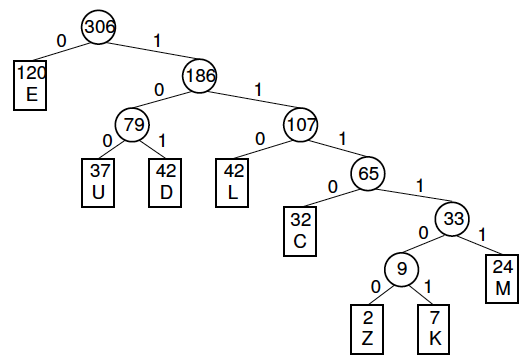
\includegraphics[width=10cm]{huffman_tree}
\end{center}

Decoding the Huffman tree is very simple, traverse the tree node by node as each bit is read from the input stream (reaching a leaf node necessarily terminates the search for that particular byte value). 

For example, decoding an encoded string can be done by looking at the bits in the coded string from left to right until a letter decoded.
10100101 $\Rightarrow$ DEED

\section{Lempel-Ziv(lz) Compression Methods}
Also known as the LZ family,it initially consisted of LZ-77 and LZ-78 which was published by Abraham Lempel and Jacob Ziv in 1977\cite{ziv1977universal} and 1978\cite{ziv1978compression}.Also known as LZ-1 and LZ-2 respectively,both are theoretically dictionary coders.These algorithms formed the basis for a lot of variations like LZW,LZSS,LZMA and also for a lot compression schemes like DEFLATE which has been discussed later in this article.


\subsection{LZ-77 Algorithm}
LZ77 algorithms achieve compression by replacing repeated occurrences of data with references to a copy of that data existing earlier within the uncompressed data stream. A match is encoded by a pair of numbers called a length-distance pair, which is like the statement "each of the next length characters is equal to the characters exactly distance characters behind it in the uncompressed stream".

To spot matches, the encoder must keep track of some amount of the recent data, like the last 2 kB, 4 kB, or 32 kB. The structure during which this data is held is named a sliding window , which is why LZ77 is usually called sliding-window compression. The encoder must keep this data to find matches, and therefore the decoder must keep this data to interpret the matches the encoder refers to. The larger the sliding window is, the longer back the encoder may look for creating references.

While encoding, for the search pointer to continue finding matched pairs after the end of the search window, all characters from the primary match at offset D and forward to the end of the search window must have matched input, and these are the (previously seen) characters that comprise one run unit of length LR, which must equal D. When search pointer proceeds past the search window and forward, as long as the run pattern repeats within the input, the search and input pointers are going to be in sync and match characters until the run pattern is interrupted. Then L characters had been matched in total, L > D, and therefore the code is [D, L, c].

Upon decoding [D, L, c], again, D = LR. When the primary LR characters are read to the output, this corresponds to one run unit appended to the output buffer. At this moment , the read pointer might be thought of as only needing to return int(L/LR) + (1 if L mod LR != 0) times to the beginning of that single buffered run unit, read LR characters (or maybe fewer on the last return), and repeat until all of the L characters are read. But mirroring the encoding process, since the pattern is repetitive, the read pointer need only trail in sync with the write pointer by a fixed distance which is equal to the run length LR until L characters are copied to output in total.

\begin{algorithm}
	\caption{LZ-77}
	\begin{algorithmic}[0]
		\WHILE{input not empty}
		\STATE prefix : longest prefix of input that begins in window
		\IF{prefix exists}
		\STATE j : distance to start of prefix
		\STATE k : length of prefix
		\STATE a : char following prefix in input
		\IF{j := 0}
		\STATE k := 0
		\STATE a := first char of input
		\ENDIF
		\ENDIF
		\STATE \textbf{output}(j, k, a)
		\STATE s := pop k + 1 char from front of input
		\STATE discard k+1 char from front of window
		\STATE append s to back of window
		\ENDWHILE
	\end{algorithmic}
\end{algorithm}



\subsection{LZ-78 Algorithm}
The LZ78 is also a dictionary-based compression algorithm that maintains a dictionary. The encoded output
consists of two elements: an index pertaining to the longest matching lexical entry and therefore the first non-matching
symbol. The algorithm also adds the index and symbol pair to the dictionary. When the symbol is not yet found in
the dictionary, the codeword has the index value 0 and it's added to the dictionary as well . With this method, the
algorithm constructs the dictionary.
LZ78 algorithm has the power to capture patterns and hold them indefinitely but it also features a serious drawback.
The dictionary keeps growing forever without bound. There are a lot of methods to limit dictionary size. the
easiest one is to stop adding entries and continue like a static dictionary coder or to throw the dictionary away and
start from scratch after a certain number of entries has been reached\cite{zeeh2003lempel}

\begin{algorithm}
	\caption{LZ-78}
	\begin{algorithmic}[0]
		\STATE q:NIL;
		\WHILE{there is input}
		\STATE j : next symbol from input
		\IF{$q_j$ exists in the dictionary}
			\STATE q : $q_j$
		\ELSE
			\STATE \textbf{output}(index(q), j)		
			\STATE Add $q_j$ to the dictionary
			\STATE q : NIL
		\ENDIF
		\ENDWHILE

	\end{algorithmic}
\end{algorithm}



\section{Arithmetic Coding}

Arithmetic coding \cite{witten1987arithmetic} is a data compression technique that encodes data (the data string) by creating a code string which represents a fractional value on the number line between 0 and 1. The coding algorithm is symbolwise recursive; i.e., it operates upon and encodes (decodes) one data symbol per iteration or recursion. On each recursion, the algorithm successively partitions an interval of the number line between 0 and 1, and retains one of the partitions as the new interval. Thus, the algorithm successively deals with smaller intervals, and the code string, viewed as a magnitude, lies in each of the nested intervals. The data string is recovered by using magnitude comparisons on the code string to recreate how the encoder must have successively partitioned and retained each nested subinterval. Arithmetic coding differs considerably from the more familiar compression coding techniques, such as prefix (Huffman) codes. Also, it should not be confused with error control coding, whose object is to detect and correct errors in computer operations.\cite{rissanen1979arithmetic} \cite{langdon1984introduction}

\begin{algorithm}
	\caption{Arithmetic Coding}
	\begin{algorithmic}[0]
		\STATE count source units
		\STATE interval I := \textbf{new} interval 0..1
		\STATE divide I according to rate of units
		\STATE \textbf{readSymbol}(X) \linebreak
		\WHILE{X != EOF}
		\STATE new I := subinterval I matching X
		\STATE divide I acording to rate of units
		\STATE readSymbol(X)
		\ENDWHILE
		\STATE \textbf{output}(best number from I)
	\end{algorithmic}
\end{algorithm}

For example, suppose the alphabet is (a, e, i, O, u, !), and a fixed model is used
with probabilities shown

\begin{table}[]
	\setlength{\extrarowheight}{0.2cm}
	\begin{tabular}{|l|l|l|}
		\hline
		Symbol & Probability & Range        \\ \hline
		a      & 0.2         & {[}0, 0.2)   \\ \hline
		e      & 0.3         & {[}0.2, 0.5) \\ \hline
		i      & 0.2         & {[}0.5, 0.7) \\ \hline
		o      & 0.1         & {[}0.7, 0.8) \\ \hline
		u      & 0.1         & {[}0.8, 0.9) \\ \hline
		!      & 0.1         & {[}0.9, 1.0) \\ \hline
	\end{tabular}
\end{table}

We have to transmit the message 'eaii!'. Initially, both encoder and decoder know that the range is [0, 1). After seeing the first symbol, e, the encoder narrows it to [0.2, 0.5), the range the model allocates to this symbol. The second symbol, a, will narrow this new range to the first one-fifth of it, since a has been allocated [0, 0.2). This produces [O.2, 0.26), since the previous range was 0.3 units long and one-fifth of that is 0.06. The next symbol, i, is allocated [0.7, 0.8),which when applied to [0.2, 0.26) gives the smaller range [0.242, 0.248). Proceeding in this way, the en-coded message builds up as follows:  

Initially [0, 1)

After seeing 

e [0.2, 0.5)
\\
a [0.2, 0.26)
\\
i [0.242, 0.248)
\\
i [0.2462, 0.2468)
\\
! [0.24674, 0.2468) \\

Suppose all the decoder knows about the message is the final range, [0.24674, 0.2468) .It can -immediately deduce that the first character was e since the range lies entirely within the space the model of Table allocates for e. Now it can simulate the operation of the encoder:

Initially [0, 1)
\\
After seeing e [0.2, 0.5)
\\

This makes it clear that the second character is a,since this will produce the range

After seeing a [0.2, 0.26),which entirely encloses the given range [0.24674, 0.2468). Proceeding like this, the decoder can identify the whole message. However, the decoder will face the problem of detecting the end of the message, to determine when to stop decoding. After all, the single number 0.0 could represent any of a, aa, aaa, aaaa, . . .  . To resolve the ambiguity, we ensure that each message ends with a special EOF symbol known to both encoder and decoder. For the alphabet of Table I, "!" will be used to terminate messages  When the decoder sees this symbol,it stops decoding. 

Relative to the fixed model of Table, the entropy
of the five-symbol message ‘eaii!’ is 

$$-\log{0.3} - \log{0.2} - \log{0.1} - \log{0.1} - \log{0.1} = -\log{0.00006} =4.22$$



\section{DEFLATE}

In computing, Deflate may be a lossless data compression file format that uses both  LZ77 and Huffman coding. It was designed by Phil Katz, for version 2 of his PKZIP archiving tool. Deflate was later specified in RFC 1951 \cite{deflate}
The deflate compressor is given an excellent deal of flexibility to compress the info . The programmer must design smart algorithms to form the proper choices, but the compressor does have choices about the way to compress data.

There are three modes of compression that the compressor has available:

\begin{enumerate}
	\item Not compressed at all. This is an intelligent choice for, say, data that's already been compressed. Data stored during this mode will expand slightly, but not as much as it would if it was already compressed and any other compression methods was tried upon it.
	
	\item Compression, first with LZ77 then with Huffman coding. The trees used to compress during this mode are defined by the Deflate specification itself and no extra space must be taken to store those trees.
	
	\item Compression, first with LZ77 then with Huffman coding with trees that the compressor creates and stores along side the data.	
\end{enumerate}

The data is choppy in ``blocks,'' and every block uses a single mode of compression. If the compressor wants to change  from non-compressed storage to compression with the trees defined by the specification, or to compression with specified Huffman trees, or to compression with a different pair of Huffman trees, the present block must be ended and another one begun.


\vspace{0.6in}

\textbf{\Large{Current Research Work}}


The current research work in Data Compression has shifted more towards the application part, where data compression is being applied in all sorts of fields like Deep Learning, Networking, Image Compression, Video and Audio Compression etc. We have discussed few papers which represent the research done in various domains to get the most out of data compression and make computing systems more efficient.

\section{Tweet Classification By Data Compression \cite{10.1145/2064448.2064473}}

The above mentioned paper proposes a compression based method for classification of tweets. They used the DEFLATE algorithm to compress the tweet and then evaluate and classify the given tweet according to its compressibility. The proposed method achieved higher accuracy when compared to the state of the art learning methods. 

\subsection{Proposed Method}

The main problem was to classify the tweet according to the sentiment of the tweet, i.e classifying them into "positive" and "negative" classes. The algorithm was fed query strings and then slow it learns the difference by creating two tweet models $M_n$ and $M_p$. Finally the algorithm calculates a classification score $f(x)$ which is then used to finally classify using a fixed threshold value.

\subsection{Classification}

There are 2 steps involved in the classification procedure. The first step calculated the compressibility of the tweet and the second step calculates the classification score. \\ 

The Compressibility scores are calculated as follows  \cite{10.1145/2064448.2064473}

$$C_p = Z(M_p . x) - Z(M_p)$$
$$C_n = Z(M_n . x) - Z(M_n)$$

Where $C_p$ and $C_n$ are the compressibility scores. $M_p . x$ implies that $x$ is appended to $M_p$ and $Z(k)$ is the compressed size of the input $k$ 

And finally the classification score is calculated as follows

$$
f(x) = \frac{C_p(x) + \gamma}{C_n(x) + \gamma}
$$

where $\gamma$ is a smoothing parameter. Also known as Laplace Smoothing. 

\subsection{Related Work}
Data compression has recently been used for data mining. Benedetto et al. used gzip for language recognition, authorship attribution, and language classification \cite{benedetto2002language}. Cilibrasi and Vit´anyi presented a method for clustering by compression, which is based on the normalized compression distance
(NCD) \cite{li2004similarity}, and reported the evidence of successful application in areas as diverse as genomics, virology, music, astronomy, etc \cite{cilibrasi2005clustering}. Bratko et al. investigated an approach to
spam filtering based on statistical data compression models, and their empirical evaluations indicated that their approach outperforms currently established spam filters based on machine learning algorithms \cite{bratko2006spam}. Marton et al. reported the effectiveness and behavior of different compression-based text classification methods on English text \cite{marton2005compression}.

On the other hand, machine learning approaches have been frequently applied to Twitter mining. Irani et al. devised machine learning methods such as the decision tree for identifying the tweets in which spammers misused
trending topics by using tweet text and the associated web
pages with the tweet \cite{irani2010study}. Sriram et al. devised a Naive Bayes
classifier for identifying tweet types such as news, events, opinions, deals, and private messages based on the author information and tweet texts \cite{sriram2010short}. Sakaki et al. devised a support vector machine for finding tweets related to an event (e.g., earthquake) \cite{sakaki2010earthquake}. To their knowledge, there was no application of data compression to Twitter mining.


\subsection{Results}

According to the results mentioned in the article, CTC performed statistically better than the state of the art methods. This method also applies to multi lingual tweets which gives it an edge over some of the other machine learning approaches.

This paper was an interesting application of the DEFLATE algorithm to classify tweets.


\section{Energy Aware Lossless Data Compression \cite{10.1145/1151690.1151692}}

This paper reports a rather different viewpoint on the whole compression domain. The energy required to send a bit via wireless transmission is close to 1000 times higher than the energy required for a regular 32 bit operation on a computer \cite{note1998writing}. The article reports the fact that compressing and decompressing information before and after transmission is more energy expensive compared to the case without any compression. The paper suggests solutions to this problem and they are able to achive an energy reduction of close to 51\%.

\subsection{Lossless Data Compression of low-bandwidth devices}
Compression algorithms are versatile. They can be applied at a lot of points in the hardware-software spectrum. When compression is applied in hardware, the benefits and costs propagate to all aspects of the system. Compression in software may
have a more dramatic effect, but for better or worse, its effects will be less global. An all-purpose header compression scheme (not confined to TCP/IP or any particular protocol) appears in \cite{lilley2000unified}. TCP/IP payloads can be compressed as well with IPComp \cite{shacham2001rfc3173}, but this can be wasted effort if data has already been compressed at the application layer.

LBFS or Low Bandwidth File System leverages the similiarities between the data stored on the client and the server, and only exchanges data blocks that differ \cite{muthitacharoen2001low}. Compression is applied before the data is transmitted. Rsync \cite{tridgell2000efficient} is a protocol for efficient file transfer which preceded LBFS. A protocol-independent scheme for text compression,
NCTCSys, is presented in \cite{motgi2001network}

Along with remote proxy servers which may cache or
reformat data for mobile clients, splitting the proxy between client and server has been proposed to implement certain types of network traffic reduction for HTTP transactions \cite{housel1996webexpress} \cite{krashinsky2003efficient}. Because the delay required for manipulating data can be small in comparison with the latency
of the wireless link, bandwidth can be saved with little
effect on user experience. Alternatively, compression
can be built into servers and clients as in the mod gzip
module available for the Apache webserver and HTTP
1.1 compliant browsers \cite{hyperspace}. Delta encoding, the transmission of only parts of documents which differ between
client and server, can also be used to compress network
traffic \cite{hunt1996empirical} \cite{mogul1999trace} \cite{mogul1997potential} \cite{santos1998increasing}


\subsection{Methodologies and Summary}
The tests were done on a Compaq Personal Server codenamed "Skiff".\cite{compaq}

The energy required for compression and decompression are almost directly proportional to time required for executing. The energy required is observed to be more for aggressively compressed data due to the large number of memory references. Even though the energy requirement is proportional to the execution time, using the fastest algorithm for compression and decompression doesn't reduce the energy footprint. They were able to conclude the fact that reducing energy is not as simple as picking the fastest compression algorithm. To facilitate such dynamic energy adjustment, they were working on EProf: a portable, realtime, energy profiler which plugs into the PC-Card socket of a portable device \cite{koskelin2002eprof}

The energy requirements of the CPU and Network change drastically. They are extremely difficult to predict over a period of time. Thus software developers have to be aware of their hardware constraints and optimize accordingly to reduce energy footprint. 

\section{Lossless Compression of Already Compressed Textures \cite{strom2011lossless}}

The following cited paper investigates and proposes a lossless compression algorithm for rendering textures in graphics

Compressing textures allow the computer to render more textures due to smaller memory consumption, as the memory access. Compared to image compression methods like JPEG however, textures codecs are typically much less efficient, which is a problem when downloading the texture over a network or reading it from disk. Therefore, in this paper we investigate lossless compression of already compressed textures. By predicting compression parameters in the image domain instead of in the parameter domain, a more efficient representation is obtained compared to using general compression such as ZIP or LZMA.



\section{On the Compressive Power of Boolean Threshold Autoencoders \cite{melkman2020compressive}}

An autoencoder is a layered neural network whose structure can be viewed as consisting of an encoder, which compresses an input vector of dimension D to a vector of low dimension d, and a decoder which transforms the low-dimensional vector back to the original input vector (or one that is very similar). In this paper they explore the compressive power of autoencoders that are Boolean threshold networks by studying the numbers of nodes and layers that are required to ensure that each vector in a given set of distinct input binary vectors is transformed back to its original\cite{ackley1985learning}. It is shown that that for any set of n distinct vectors there exists a seven-layer autoencoder with the smallest possible middle layer, (i.e., its size is logarithmic in n), but that there is a set of n vectors for which there is no three-layer autoencoder with a middle layer of the same size. In addition we present a kind of trade-off: if a considerably larger middle layer is permissible then a five-layer autoencoder does exist. The results obtained suggest that it is the decoding that constitutes the bottleneck of autoencoding. For example, there always is a three-layer Boolean threshold encoder that compresses n vectors into a dimension that is reduced to twice the logarithm of n.\cite{anderson1988neurocomputing} \cite{kingma2013auto} \cite{doersch2016tutorial}




\section{Texture compression using low-frequency signal modulation \cite{10.5555/844174.844187}}

A new lossy texture compression technique is presented in this paper that is suited to implementation on low-cost, low-bandwidth devices as well as more powerful rendering systems. It uses a representation that is based on the blending of two (or more) 'low frequency' signals using a high frequency but low precision modulation signal. Continuity of the low frequency signals helps to avoid block artifacts. Decompression costs are kept low through use of fixed-rate encoding and by eliminating indirect data access.


\section{Conclusion and Future Prospects}

In the presented review article we had an overview and simple examples of some of the most established methods in the domain of Lossless Data Compression. We also had a look at some of the modern research going on in the field. Almost every software system in function today has a component of compression and decompression to reduce the load and improve efficiency. 

When large groups of similar files are stored, such as a group of sequential videos, they can be combined into archive files. Archive files don't have to be compressed, but they are often several gigabytes in size, so they are usually compressed to save storage space and transmission time. Most compression programs also have the ability to archive files into one large file. Most operating systems will compress their backup files, which are very large archive files, since these files just take up space until the need for them arises.

As we are moving towards a more data driven age, the amount of which users are creating data is exploding. In such scenarios, data compression stands at a very crucial juncture. Active research in this field will yield astonishing speed improvements in the current computing landscape.

\clearpage

\bibliographystyle{unsrt}
\bibliography{main}

\end{document}